%\newpage
%\subsection{Dataset}

Next, we apply our method to brain imaging data from the anonymized multimodal
neuroimaging ``Mother Of all Unification Studies'' (MOUS) dataset
\citep{schoffelen2019204}. The dataset contains magneto-encephalography (MEG)
recordings of 102 healthy native-Dutch adults who participated in a reading
task. Twelve subjects were excluded from the analysis because of corrupted file headers.
%
Subjects were exposed to a rapid serial visual presentation of Dutch words. The
word lists consisted of 120 sentences, and scrambled lists of the same words.
Each word was presented on the computer screen for 351ms on average (min: 300ms,
max: 1400ms). Successive words were separated by a blank screen for 300ms, and
successive sentences were separated by an empty screen for a few (3-4) seconds.

\subsubsection{MEG preprocessing}

The raw MEG data was bandpass-filtered between 0.1 and 40Hz using MNE-Python
default parameters \citep{gramfort2013meg, gramfort2014mne}. Specifically, we used a zero-phase finite impulse
response filter (FIR) with a Hamming window and with transition bands of 0.1Hz
and 10Hz for the low and high cut-off frequencies. The raw data was then segmented 100ms before word onset and 1s after
word onset ($t=0$ms corresponds to word onset). Finally, each resulting
segment was baseline-corrected between -100ms and 0ms, and decimated by 5 and
thus led a sampling frequency of 240Hz. The average responses across words is displayed in Figure \ref{fig:meg_evoked}.
For each subject and each time sample relative to word onset, we
build an observation matrix $Y \in \mathbb{R}^{n \times d_y}$ of $n\approx$ 2700 words
by $d_y=301$ MEG channels (273 magnetometers and 28 compensation channels). Each
of the columns of $Y$ is normalized to have zero mean and unit variance.

\begin{figure}[t!]
  \begin{minipage}[c]{0.6\textwidth}
    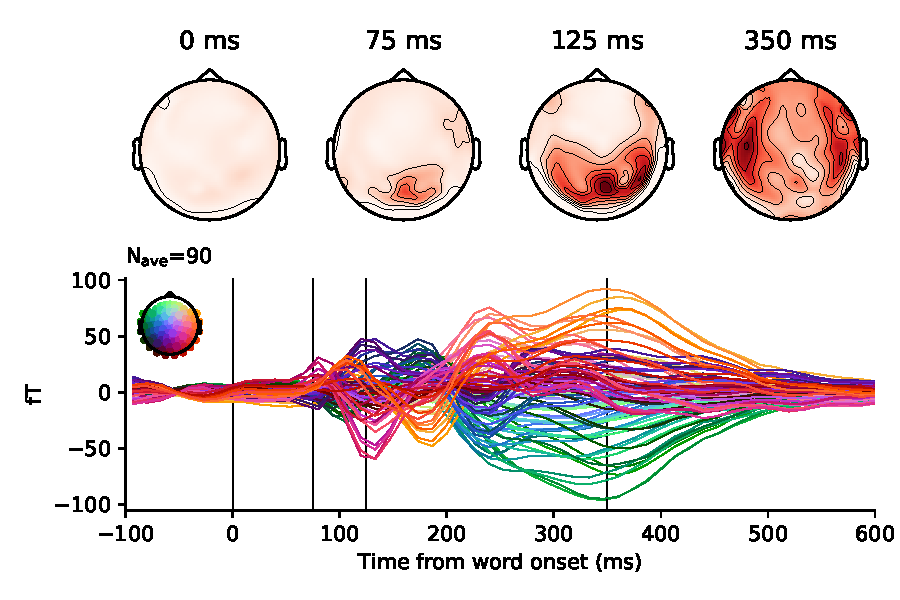
\includegraphics[width=\textwidth, trim=0cm 0cm 0cm 0cm, clip=True]{figures/meg_evoked.pdf}
  \end{minipage}\hfill
  \begin{minipage}[c]{0.4\textwidth}
    \caption{Ninety subjects read approximately 2,700 words while their brain activity was recorded with MEG. Top. Average brain response to words (word onset at t=0 ms), as viewed from above the head (red= higher gradient of magnetic flux). Bottom. Each line represents magnetometer, color-coded by spatial position. Posterior responses, typical of primary visual cortex activity, peak around 100 ms after word onset and are followed by an anterior propagation of activity typical of semantic processing in the associative cortices.
    }
    \label{fig:meg_evoked}
  \end{minipage}
\end{figure}


\subsubsection{Feature definition}

We aim to identify the word features that cause a variation in brain responses. We consider four distinct but colinear features.
%
First, 'Word Length' refers to the total number of letters. Word Length is expected to specifically cause a variation in the early evoked MEG responses (i.e. from 100 ms after stimulus onset) elicited by the retinotopically-tuned visual cortices (e.g. \citep{pegado2014timing}.).
%
Second, 'Word Frequency' indexes how frequently each word appears in Dutch and was derived with the the Zipf logarithmic scale of \citep{van2014subtlex} provided by the WordFreq package \citep{speerwordfreq}. Word Frequency is expected to specifically cause a variation in the late evoked MEG responses (i.e. from 400 ms), because it variably engages semantic processes in the temporal cortices \citep{kutas2011thirty}.
%
Third, 'Word Function' indicates whether each word is a content word (i.e. a noun, a verb, an adjective or an adverb) or a function word (i.e. a preposition, a conjunction, a determinant, a pronoun or a numeral), and was derived from Spacy's part of speech tagger \citep{spacy2}. To our knowledge, this feature has not been thouroughly investigated with MEG. Its causal contribution to reading processes in the brain thus remains unclear.
%
Finally, to verify that B2B and other methods would not inadequately identify non-causal features, we added a dummy feature, constructed from a noisy combination of Word Length and Word Frequency:
$dummy = z(length) + z(frequency) + \mathcal{N}$, where $z$ normalizes features and $\mathcal{N}$ is a random vector sampling Gaussian distribution (all terms thus have a zero-mean and a unit-variance).

This procedure yields an $X \in \mathbb{R}^{n \times d_x}$ matrix of $n\approx$ 2700 words by
$d_x=4$ features for each subject. Each of the columns of $X$ is normalized to
have a mean and a standard deviation of 0 and 1 respectively.

\subsubsection{Models and statistics}

We compare B2B to four standard methods: Forward regression, Backward regression, CCA and PLS, as implemented in scikit-learn \citep{sklearn}, and optimized with nested cross validation over twenty $l2$ regularization parameters logarithmically spaced between $10^{-4}$ and $10^4$ (for regression methods) or 1 to 4 canonical components (for cross-decomposition methods).

We used the feature importance described in Algorithm \ref{algorithm:b2b_fi} to assess the extent to which each feature $X_i$ specifically improves the prediction of held-out $Y$ data, using a 5-fold cross-validation (with shuffled trials to homogeneize the distributions between the training and testing splits).

Each model was implemented for each subject and each time sample independently. Pairwise comparison between models were performed using a Wilcoxon test across subjects (n=90) using the average $\Delta R$ across time.

Corresponding results are shown in Figure~\ref{fig:meg_results}.



\begin{wrapfigure}{r}{.5\textwidth}
  \vspace{-12ex}
  \begin{center}
    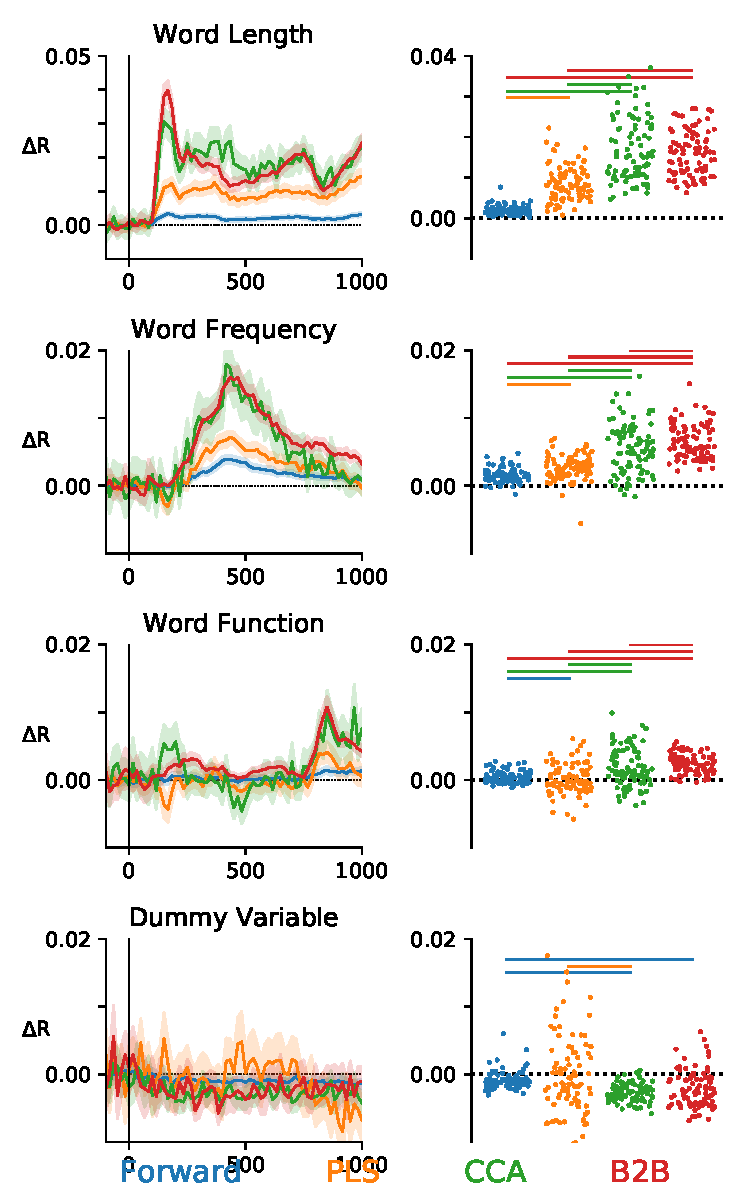
\includegraphics[width=0.48\textwidth, trim=0cm 0cm 0cm 0cm, clip=True]{figures/meg.pdf}

    \label{fig:meg_results}
  \end{center}
  \caption{Multiple models (color-coded) are compared on their ability to reliably predict single-trial MEG signals evoked by words. Left. Average improvement of correlation coefficient $\Delta R$ for each of the four features (rows). Error bars indicate standard error of the mean (SEM) across subjects. Right. Average $\Delta R$ across time for each subject (dot). Top horizontal lines indicate when B2B significantly outperforms other methods.}
  \vspace{-9ex}
\end{wrapfigure}

\subsubsection{Results}
We compared the ability of Forward regression, Backward regression, CCA, PLS and B2B to estimate the causal contribution of four distinct but collinear features on brain evoked responses to words.

Supplementary Figure \ref{fig:meg_supp} shows that the Backward model decodes the dummy variable well above chance level. In addition, the Backward model reveal a similar decoding time course for Word Length and Word Frequency, even though these features are known to specifically influence early and late MEG responses respectively \citep{kutas2011thirty}. These results illustrate that backward modelling cannot be used to estimate the causal contribution of collinear features.

We thus focus on the four remaining methods (i.e. Forward Regression, PLS, CCA, and B2B) and estimate their $\Delta R$ (i.e. the improvement of Y prediction induced by the introduction of a given feature into the model \ref{algorithm:b2b_fi}). Contrary to the Backward Model, none of the models predicted the Dummy Variable to improve the $Y$ prediction: all $\Delta R < 0$ (all $p > .089$).

Figure \ref{fig:meg_results} shows, for each model, the effects obtained across time (left) and subjects (right).

Word Length and Word Frequency improved the prediction performance of all methods: $\Delta R>0$ for all models (all $p<0.0001$). As expected, the time course associated with Word Length and Word Frequency rose from $\approx$ 100 ms and from $\approx$ 400 ms respectively. Furthermore, Word Function improved the prediction performance of all models (all $p < 0.0002$) except for PLS~($p=0.7989$). Overall, these results confirm that Word Length, Word Frequency and Word Function causally influence specific periods of brain responses to words.

To assess which model would be most sensitive to these causal discoveries, we compared B2B to other models across subjects (Figure \ref{fig:meg_results} right). For Word Length B2B outperforms all models (all $p < 0.00001$) but CCA ($p=0.0678$). For Word Frequency, B2B outperforms all models (all $p < 0.0006$). For "Word Function", B2B outperforms all models (all $p < 0.0015$). Overall, these results show that B2B reliably outperform standard methods, especially when the effects are difficult to detect.
